\documentclass[t,11pt]{beamer}
\usepackage{tikz}
\usepackage{pgfplots}
\usetikzlibrary{calc}
\usepackage[utf8]{inputenc}
\usepackage[ngerman]{babel}
\usepackage{amsmath,amsfonts,amssymb}
\usepackage{framed}
\usecolortheme{orchid}
\usepackage{etoolbox}
\useinnertheme[shadow=true]{rounded}

%%% PROGRESSBAR
\definecolor{pbblue}{HTML}{D8D8D8}% filling color for the progress bar
\definecolor{pbgray}{HTML}{F2F2F2}% background color for the progress bar
\useoutertheme{infolines}
\setbeamerfont{footline}{size=\normalsize}
\setbeamersize{text margin left=30pt,text margin right=30pt}
\makeatletter
\setbeamertemplate{footline}
{
	\leavevmode%
	\hbox{%
		\begin{beamercolorbox}[wd=.333333\paperwidth,ht=2.5ex,dp=1ex,center]{title in head/foot}%
			\usebeamerfont{title in head/foot}\insertshorttitle
		\end{beamercolorbox}%
		\begin{beamercolorbox}[wd=.333333\paperwidth,ht=2.5ex,dp=1ex,center]{date in head/foot}%
			%\usebeamerfont{date in head/foot}\insertshortdate{}\hspace*{2em}
			%\insertframenumber\hspace*{2ex} 
		\end{beamercolorbox}
		\begin{beamercolorbox}[wd=.333333\paperwidth,ht=3ex,dp=1ex,center]{author in head/foot}%
			\usebeamerfont{author in head/foot}\insertshortauthor~~%\beamer@ifempty{\insertshortinstitute}{}{(\insertshortinstitute)}
		\end{beamercolorbox}%
	}%
	\vskip0pt%
}
\makeatother
\makeatletter
\def\progressbar@progressbar{} % the progress bar
\newcount\progressbar@tmpcounta% auxiliary counter
\newcount\progressbar@tmpcountb% auxiliary counter
\newdimen\progressbar@pbht %progressbar height
\newdimen\progressbar@pbwd %progressbar width
\newdimen\progressbar@tmpdim % auxiliary dimension
\progressbar@pbwd=\linewidth
\progressbar@pbht=1.5ex
\def\progressbar@progressbar{%
    \progressbar@tmpcounta=\insertframenumber
    \progressbar@tmpcountb=\inserttotalframenumber
    \progressbar@tmpdim=\progressbar@pbwd
    \multiply\progressbar@tmpdim by \progressbar@tmpcounta
    \divide\progressbar@tmpdim by \progressbar@tmpcountb
  \begin{tikzpicture}[rounded corners=3pt,very thin]
    \shade[top color=pbgray!20,bottom color=pbgray!20,middle color=pbgray!50]
      (0pt, 0pt) rectangle ++ (\progressbar@pbwd, \progressbar@pbht);
      \shade[draw=pbblue,top color=pbblue!50,bottom color=pbblue!50,middle color=pbblue] %
        (0pt, 0pt) rectangle ++ (\progressbar@tmpdim, \progressbar@pbht);
    \draw[color=normal text.fg!50]  
      (0pt, 0pt) rectangle (\progressbar@pbwd, \progressbar@pbht) 
        node[pos=0.5,color=normal text.fg] {\textnormal{%
             \pgfmathparse{\insertframenumber*100/\inserttotalframenumber}%
             \pgfmathprintnumber[fixed,precision=0]{\pgfmathresult}\,\%%
        }%
    };
  \end{tikzpicture}%
}
\addtobeamertemplate{headline}{}
{%
  \begin{beamercolorbox}[wd=\paperwidth,ht=4ex,center,dp=1ex]{white}%
    \progressbar@progressbar%
  \end{beamercolorbox}%
}
\makeatother


%%% BLOCKS
% block = Aufgabe
\setbeamercolor{block title}{fg=black,bg=blue!30!white} 
\setbeamercolor{block body}{fg=black, bg=blue!3!white}

% alertblock = Definition
\setbeamercolor{block title alerted}{fg=black,bg=red!50!white} 
\setbeamercolor{block body alerted}{fg=black, bg=red!3!white}

% exampleblock = Wiederholung
\setbeamercolor{block title example}{fg=black,bg=green!30!white} 
\setbeamercolor{block body example}{fg=black, bg=green!3!white}



\begin{document}
	%\author{www.oilbat.de}
	%\title{Stochastik}
	\subtitle{}
	\logo{}
	\institute{}
	\date{}
	\subject{}
	\setbeamercovered{transparent}
	\setbeamertemplate{navigation symbols}{}

\addtocounter{framenumber}{-1}
\setbeamercovered{invisible}

\begin{frame}
	\begin{block}{Aufgabe}
		Die Dichte einer stetigen Zufallsvariable $X$ ist gegeben durch
		\begin{align*}
			f(x)=\begin{cases}
			\frac{1}{4}+c\cdot x & 0<x<1\\
			0 & \text{sonst}
			\end{cases},~\text{wobei}~c>0.
		\end{align*}
		\begin{enumerate}
			\item Zeige, dass $c=\frac{3}{2}$.
			\item Bestimme die Verteilungsfunktion $F(x)$.
			\item Wie sehen $f(x)$ und $F(x)$ aus?
			\item Wie groß ist $F(0,5)$?
			\item Was ist der Median, was der Erwartungswert von $X$?
		\end{enumerate}
	\end{block}
\end{frame}

\begin{frame}
	\begin{alertblock}{Definition: Dichte}
		Die Funktion $f$ ist eine Dichte, falls 
		\begin{enumerate}
			\item $f(x)\geq 0$ für alle $x$
			\item und $\int_{-\infty}^{+\infty} f(x)dx = 1$.
		\end{enumerate}
	\end{alertblock}
\end{frame}

\begin{frame}
\begin{alertblock}{Definition: Dichte}
	Die Funktion $f$ ist eine Dichte, falls 
	\begin{enumerate}
		\item $f(x)\geq 0$ für alle $x$
		\item und $\int_{-\infty}^{+\infty} f(x)dx = 1$.
	\end{enumerate}
\end{alertblock}
\begin{align*}
1 = \int_{-\infty}^{+\infty} f(x)dx &= \int_{0}^{1} \frac{1}{4}+c\cdot x~dx \\
&= \left[ \frac{1}{4}x + \frac{1}{2}cx^2 \right]^1_0  \\
&= \frac{1}{4}+\frac{1}{2}c \\
\Rightarrow c = \frac{3}{2}
\end{align*}
\end{frame}

\begin{frame}
	\begin{block}{Dichte}
		\vspace{-0.5cm}
		\begin{align*}
		f(x)=\begin{cases}
		\frac{1}{4}+\frac{3}{2} x & 0<x<1\\
		0 & \text{sonst}
		\end{cases}
		\end{align*}
	\end{block}
\end{frame}

\begin{frame}
\begin{block}{Dichte}
	\vspace{-0.5cm}
	\begin{align*}
	f(x)=\begin{cases}
	\frac{1}{4}+\frac{3}{2} x & 0<x<1\\
	0 & \text{sonst}
	\end{cases}
	\end{align*}
\end{block}
\begin{center}
	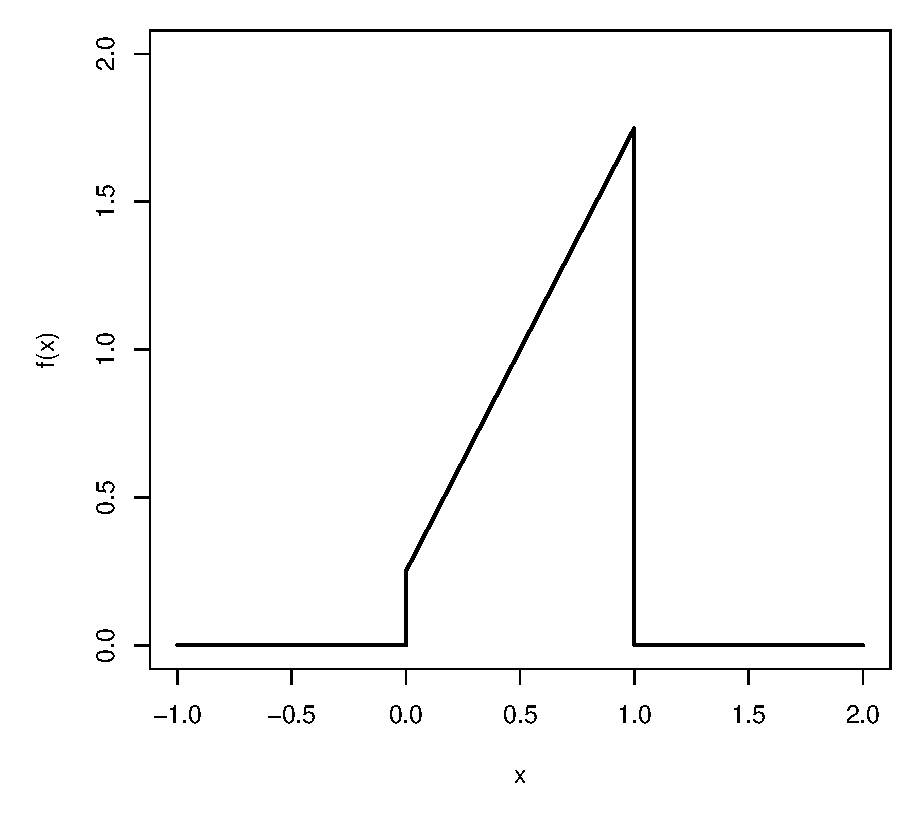
\includegraphics[scale=0.45]{f.pdf}
\end{center}
\end{frame}

\begin{frame}
	\begin{alertblock}{Definition: Verteilungsfunktion}
		Gegeben eine Dichte $f$, dann ist die zugehörige Verteilungsfunktion 
		\begin{align*}
			F(x) = \int_{-\infty}^{x} f(t)dt.
		\end{align*}
	Sie hat folgende Eigenschaften:
	\begin{enumerate}
		\item $F$ ist monoton steigend,
		\item $\lim_{x\to -\infty} F(x)=0$,
		\item $\lim_{x\to +\infty} F(x)=1$.
	\end{enumerate}
\end{alertblock}
\end{frame}

\begin{frame}
\begin{block}{Dichte}
	\vspace{-0.5cm}
	\begin{align*}
	f(x)=\begin{cases}
	\frac{1}{4}+\frac{3}{2} x & 0<x<1\\
	0 & \text{sonst}
	\end{cases}
	\end{align*}
\end{block}

\begin{block}{Verteilungsfunktion}
	\vspace{-0.5cm}
	\begin{align*}
	F(x)=\begin{cases}
	0 & x\leq 0 \\
	?  & 0<x<1\\
	1 & x \geq 1
	\end{cases}
	\end{align*}
\end{block}
\end{frame}

\begin{frame}
\begin{block}{Dichte}
	\vspace{-0.5cm}
	\begin{align*}
	f(x)=\begin{cases}
	\frac{1}{4}+\frac{3}{2} x & 0<x<1\\
	0 & \text{sonst}
	\end{cases}
	\end{align*}
\end{block}

\begin{block}{Verteilungsfunktion}
	\vspace{-0.5cm}
	\begin{align*}
	F(x)=\begin{cases}
	0 & x\leq 0 \\
	?  & 0<x<1\\
	1 & x \geq 1
	\end{cases}
	\end{align*}
\end{block}

Für $0<x<1$:
\begin{align*}
	? &= \int_{0}^{x} f(t)~dt =  \int_{0}^{x} \frac{1}{4}+\frac{3}{2} t ~dt \\
	&= \frac{1}{4}x +\frac{3}{4}x^2
\end{align*}
\end{frame}

\begin{frame}
	\begin{block}{Verteilungsfunktion}
		\vspace{-0.5cm}
		\begin{align*}
		F(x)=\begin{cases}
		0 & x\leq 0 \\
		\frac{1}{4}x +\frac{3}{4}x^2  & 0<x<1\\
		1 & x \geq 1
		\end{cases}
		\end{align*}
	\end{block}
	\begin{center}
		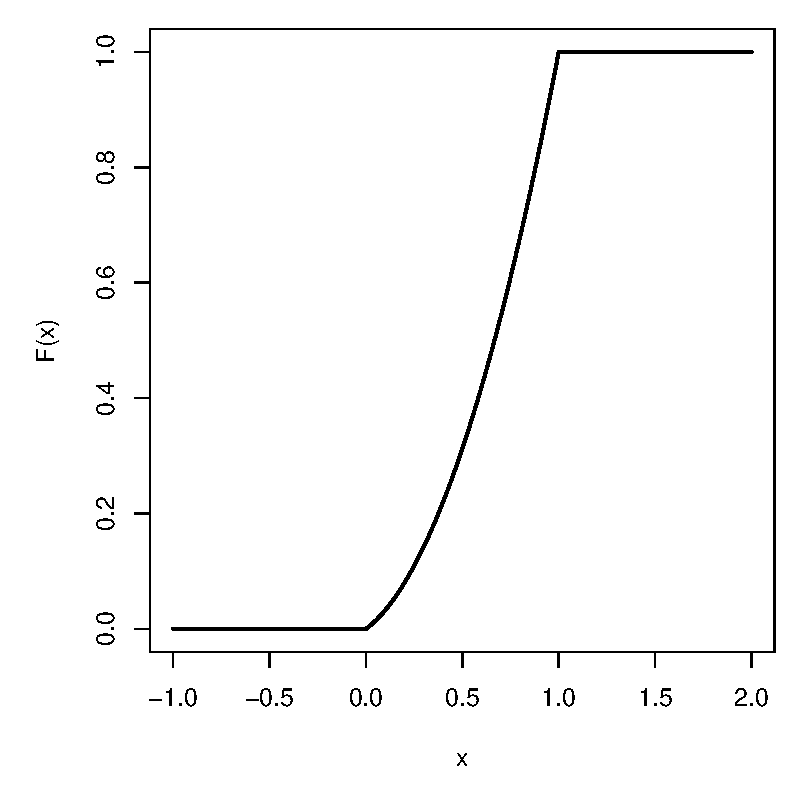
\includegraphics[scale=0.4]{Fx.pdf}
	\end{center}
\end{frame}

\begin{frame}
\begin{block}{Verteilungsfunktion}
	\vspace{-0.5cm}
	\begin{align*}
	F(x)=\begin{cases}
	0 & x\leq 0 \\
	\frac{1}{4}x +\frac{3}{4}x^2  & 0<x<1\\
	1 & x \geq 1
	\end{cases}
	\end{align*}
\end{block}
\begin{center}
	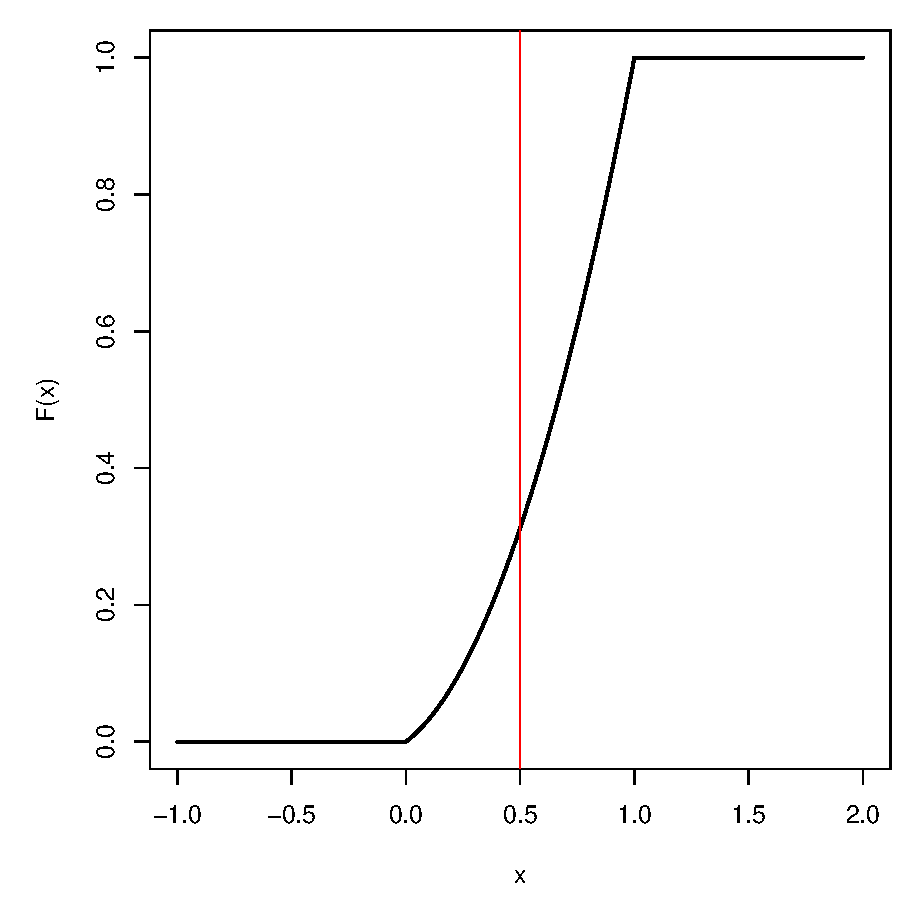
\includegraphics[scale=0.25]{Fx2.pdf}
\end{center}
$F(0,5)=\frac{1}{4}\cdot 0,5 + \frac{3}{4}\cdot 0,5^2 = 0,3125$
\end{frame}

\begin{frame}
\begin{alertblock}{Definition: Median}
	Gegeben eine stetige Verteilungsfunktion $F$, dann ist der Median der Punkt $x$, so dass 
	\begin{align*}
	F(x) = 0,5.
	\end{align*}
\end{alertblock}
\begin{center}
	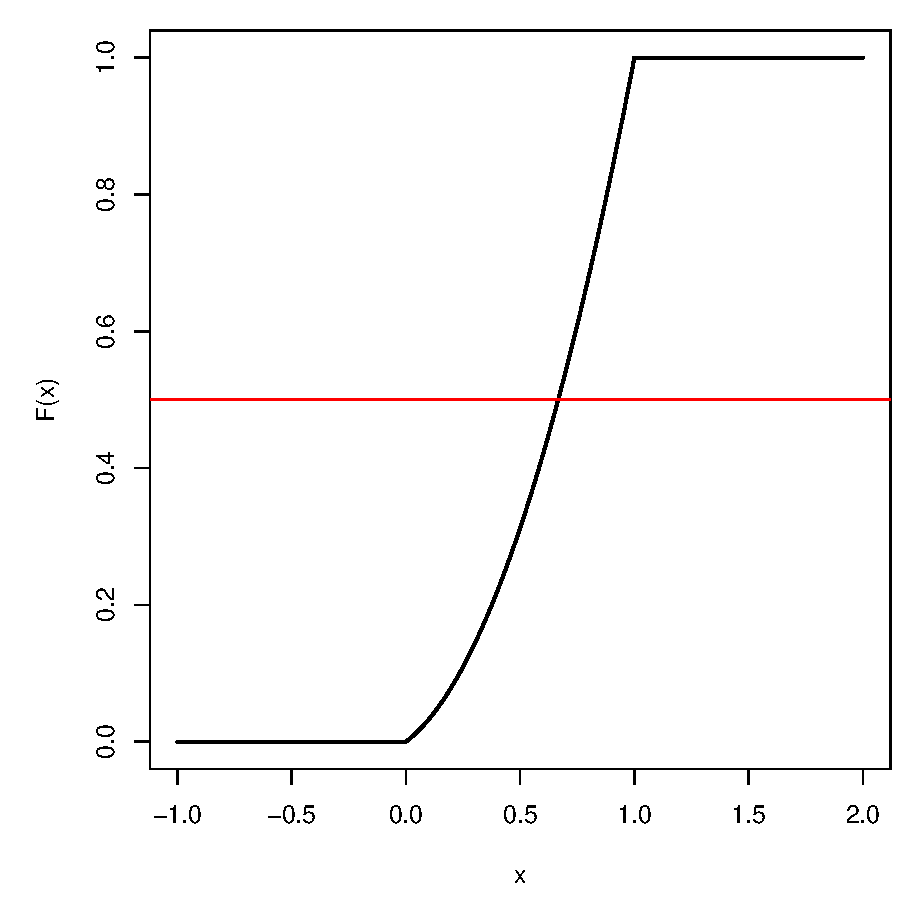
\includegraphics[scale=0.25]{Fx3.pdf}
\end{center}
$F(x)=0,5 \Rightarrow \frac{1}{4}x + \frac{3}{4}x^2 = 0,5 \Rightarrow x=\frac{2}{3}$
\end{frame}

\begin{frame}
\begin{alertblock}{Definition: Erwartungswert}
	Gegeben eine Dichte $f$, dann ist der Erwartungswert
	\begin{align*}
	\int_{-\infty}^{\infty} xf(x)~dx.
	\end{align*}
\end{alertblock}
\begin{block}{Dichte}
	\vspace{-0.5cm}
	\begin{align*}
	f(x)=\begin{cases}
	\frac{1}{4}+\frac{3}{2} x & 0<x<1\\
	0 & \text{sonst}
	\end{cases}
	\end{align*}
\end{block}
\begin{align*}
	\int_{-\infty}^{\infty} xf(x)~dx = \int_{0}^{1} \frac{1}{4}x+\frac{3}{2}x^2~dx=\left[ \frac{1}{8}x^2 + \frac{3}{6}x^3  \right]_0^1 = \frac{5}{8} 
\end{align*}

\end{frame}


\end{document}